\documentclass[12pt,a4paper]{article}
\usepackage[utf8]{inputenc}
\usepackage[spanish]{babel}
\usepackage[left=2cm,right=2cm,top=2cm,bottom=2cm]{geometry}
\usepackage{amsmath}
\usepackage{amsfonts}
\usepackage{amssymb}
\usepackage{lmodern}
\usepackage{amsmath}
\usepackage{enumerate}
\usepackage{algorithmic}
\usepackage{algorithm}
\usepackage{graphicx}
\usepackage{mathtools}

\newcommand{\LINECOMMENT}[1]{\STATE \(\triangleright\) #1}
\newcommand{\RESET}[1]{\STATE Reset: #1}
\def\BState{\State\hskip-\ALG@thistlm}

\begin{document}

\begin{titlepage}
  \begin{figure}[htb]
    \begin{center}
      
\includegraphics[width=10cm]{graphics/logo_unc.png}
      \rule{100mm}{0.1mm} \\
    \end{center}
  \end{figure}

  \begin{center}
    \vspace{15mm}
    \begin{Huge}
      Modelos y Simulaciones \\
      2017 \\
    \end{Huge}
  \end{center}

  \vspace{7mm}
  \begin{center}
    \begin{Large}
      \textbf{TRABAJO ESPECIAL}
    \end{Large}
  \end{center}

  \vspace{10mm}
  \begin{Large}
    \parindent=15mm
    \textbf{Docentes:}
    $\;$Kisbye, Patricia
    \parindent=48mm
    \par Sánchez, Jorge

    \vspace{7mm}
    \parindent=15mm
    \textbf{Alumnos:}
    $\;$Curto, Agustín
    \parindent=48mm
    \par Nievas, Francisco
  \end{Large}

  \vspace{25mm}
  \begin{figure}[htb]
    \begin{center}
      \rule{100mm}{0.1mm}
      \vspace{10mm}
      
\includegraphics[width=7cm]{graphics/logo_famaf.png}
    \end{center}
  \end{figure}
\end{titlepage}


\tableofcontents

\section{\textbf{Introducción}}

	\par Un lavadero de ropa automático, cuenta con \textbf{N} máquinas lavadoras en servicio y con \textbf{S} de
	repuesto, todas ellas de idéntica marca, modelo y antigüedad. Además el lavadero cuenta con los servicios de técnicos
	que reparan las máquinas. Obviamente, los técnicos reparan las máquinas en serie, encargándose de una sola por
	vez. El problema consiste en determinar el tiempo medio (\textit{y su correspondiente desviación estándar}) que
	transcurre hasta que el lavadero deja de ser operativo (\textit{fallo del sistema}), esto es, el momento en el que se
	tiene menos de \textbf{N} máquinas en servicio, o lo que es lo mismo, posee más de \textbf{S} máquinas defectuosas en
	el taller.

	\par Todos los tiempos de funcionamiento de las máquinas, hasta descomponerse son variables independientes
	exponenciales con un tiempo medio, hasta fallar, de \textbf{$T_{F}$} y el tiempo de reparación de una máquina que
	ingresa al taller es una variable exponencial con media igual a \textbf{$T_{R}$}, independiente de todos los
	anteriores.

	\par Se analizan dos posibles mejoras al sistema de la lavandería, en una de ellas se considera el caso en el cual el
	lavadero tiene a su disposición un operario más que al principio, y otro donde se cuenta con una máquina de repuesto
	extra.

	\par El procedimiento para poder solucionar este problema consiste de una simulación mediante un algoritmo, el cual,
	por medio de los tiempos de falla y reparación de las máquinas, realiza una recopilación de datos para luego estimar
	la media y la desviación estándar muestrales. Posterior a las estimaciones, se realizan gráficos con los datos
	recolectados y por medio de los mismos se decide que tan precisas fueron las simulaciones.


\pagebreak

\section{Algoritmo y descripción de las variables}

  \par En la siguiente sección se presentarán los algoritmos utilizados para la realización de las simulaciones del
  problema de la lavandería. Dichos algoritmos serán explicados con palabras para facilitar la comprensión del lector
  y luego se proveerá un pseudocódigo de los mismos.

  \vspace{5mm}
  \par El siguiente algoritmo simula el sistema de la lavandería, con $N$ máquinas en funcionamiento, $S$ máquinas de
  repuesto y $Op$ operarios. Para poder resolver los problemas presentados en la introducción, debemos tomar los
  siguientes valores:

  \begin{itemize}
    \item Problema 1: N = 5, S = 2, Op = 1
    \item Problema 2: N = 5, S = 2, Op = 2
    \item Problema 3: N = 5, S = 3, Op = 1
  \end{itemize}

  \par Dentro del algoritmo antes mencionado, se utilizan las siguientes variables, las cuales son inicializadas al
  comienzo del mismo:
  \begin{itemize}
    \item $time$: Variable de tiempo actual.
    \item $machines\_down\_number$: Cantidad de máquinas rotas.
    \item $repair\_time$: Lista con los tiempos de reparación de cada máquina.
    \item $life\_times$: Lista con los tiempos de vida de cada máquina, es decir, el tiempo hasta presentar una falla.
  \end{itemize}

  \par El estado del sistema puede cambiar en dos posibles casos: se averió una máquina y debe ser reemplazada, o bien,
  se terminó de reparar una máquina y la misma puede volver a ser utilizada. Para poder saber cual de dichos eventos
  ocurrió necesitamos mantener como invariante el orden de las listas $repair\_time$ y $life\_times$. A continuación
  serán explicados los dos posibles sucesos.

  \par Para resolver el primer incidente basta con verificar que el tiempo de vida de la primera máquina sea menor al
  primer tiempo de reparación, y de ser así, almacenar en la variable $time$, el tiempo de falla de la primera máquina,
  aumentando la cantidad de máquinas rotas en uno (dado que otra máquina falló). Si no existiesen máquinas de repuesto
  se terminará la simulación, puesto que el sistema no puede continuar. En caso de que existan, se genera una variable
  aleatoria $X \sim \mathcal{E}(1/T_F)$, la misma será el tiempo de falla de la nueva máquina, luego se agrega el valor
  $time + X$ a la lista $life\_time$ y se reordena dicha lista. Podría ocurrir que exista un operario libre entonces se
  le encarga la reparación de la máquina en forma inmediata, para ello se genera una variable aleatoria
  $Y \sim \mathcal{E}(1/T_R)$ y se agrega el tiempo $time + Y$ a la lista $repair\_time$, reordenando la
  misma.

  \par En el segundo incidente, se terminó de reparar una máquina por lo tanto se decrementa en uno
  $machines\_down\_number$. Además la variable $time$ será el tiempo de reparación de la primera máquina. Por otro
  lado, se calcula la cantidad de operadores libres, en caso de que hubiesen máquinas descompuestas y operarios libres
  se designa a los trabajadores dichas máquinas. Para ello, igual que en el caso anterior, se generan variables
  aleatorias $Y \sim \mathcal{E}(1/T_R)$ para cada máquina a reparar. Por último, se reordenan los valores en
  $repair\_time$ nuevamente.


  \begin{algorithm} [H]
    \caption{Experimento con $N$ máquinas en funcionamiento, $S$ de repuesto y $Op$ operarios}
    \label{alg1}
    \begin{algorithmic} [1]
    \STATE $ time \leftarrow  0 $ \label{line:1}\hfill\COMMENT{Actual time}
    \STATE $ machines\_down\_number \leftarrow  0 $ \label{line:2}
    \STATE $ repair\_time \leftarrow  \{\infty, \infty, \dots, \infty_{Op}\} $ \label{line:3}
    \STATE $ life\_times \leftarrow \{ X_1, X_2, \dots , X_N \} $ \label{line:4}
    \hfill\COMMENT{$ X_i \sim \mathcal{E}(1/T_F) $ y $ X_1 < X_2 < \dots < X_N $}

    \WHILE{System is working}
      \IF{$ life\_times_1 < repair\_time_1 $} \label{line:6}
        \RESET $ time \leftarrow  life\_times_{1}$ \label{line:7}
        \STATE $ machines\_down\_number \leftarrow  machines\_down\_number + 1 $ \label{line:8}

        \IF{$ machines\_down\_number = S + 1$}
          \RETURN $ time $ \label{line:10}
        \ENDIF
        \IF{$ machines\_down\_number < S + 1 $}
          \STATE $ X \leftarrow time + \mathcal{E}(1/T_F) $
          \STATE $ life\_times \leftarrow \{X_2, \dots, X_N, X\} $
          \STATE Reorder the values ${ X_2, \dots, X_N, X} $
        \ENDIF
        \IF{$ operator\ not\ working $}
          \STATE $ Y \leftarrow time + \mathcal{E}(1/T_F) $
          \STATE $ repair\_time \leftarrow \{X_1, \dots,\ Y, \dots, X_N, Y\} $
        \ENDIF

      \ELSE
        \RESET $ time \leftarrow repair\_time_1 $
        \STATE $ repair\_time \leftarrow \{ Y_2, Y_3, \dots, Y_N, \infty \} $
        \STATE $ free\_op \leftarrow Number\ of\ free\ operator\ $
        \IF{$ free\_op \leq machines\_down\_number $}
            \STATE $ repair\_times \leftarrow \{ time + Y_1, time + Y_2, \dots, time + Y_N \} $
                \hfill\COMMENT{$ Y_i \sim \mathcal{E}(1/T_r)$}
            \STATE $ free\_op \leftarrow 0 $
        \ENDIF
        \IF{$ machines\_down\_number = 0 $}
          \STATE $ repair\_times \leftarrow \{ \infty, \infty, \dots, \infty \} $
        \ENDIF
        \IF{$ 0 < machines\_down\_number < free\_op $}
          \STATE $ repair\_times \leftarrow \{ time + Y_1,\dots, time + Y_{free\_op}, \infty,\dots\} $
          \hfill\COMMENT{$ Y_i \sim \mathcal{E}(1/T_r)$}

        \ENDIF
        \STATE Reorder the values in $ repair\_time $
      \ENDIF
    \ENDWHILE
    \end{algorithmic}
  \end{algorithm}

  \pagebreak
  \par El algoritmo posterior se encarga de simular el experimento propiamente dicho, es decir, recrear la simulación
  la cantidad de veces necesarias para obtener los valores de la media y varianza muestrales de los tiempos de vida del
  sistema, con un nivel de confianza $\alpha$.

  \begin{algorithm}
  \caption{Simulación del experimento con confianza $\alpha$}
    \label{alg2}
    \begin{algorithmic}
      \STATE Elegir $\alpha$ como valor aceptable de $\sigma / \sqrt{n}$
      \STATE Generar al menos 1000 valores de X.
      \WHILE{$S(n) /\sqrt{n} > \alpha$}
        \STATE $n \leftarrow n + 1$
        \STATE Simular $X$ con el experimento
      \ENDWHILE
      \RETURN $\overline{X}(n)$
    \end{algorithmic}
  \end{algorithm}


\pagebreak

\section{Resultados}

  \par En esta sección se presentarán resultados de las simulaciones realizadas. Se realizarán histogramas
  comparativos entre las distintas simulaciones. Dichos gráficos serán explicados y analizados brevemente en esta
  sección y con mayor detalle en la siguiente.

  \par Como comentario general de los histogramas, vale aclarar que se proyectará sobre el eje de las abcisas la
  durabilidad del sistema en meses. Mientras que en el eje de las ordenadas al origen graficaremos las frecuencias
  relativas de los valores obtenidos por la simulación.

  \par Cabe recordar, los valores de las variables para la simulación mediante los algoritmos anteriormente descritos,
  para cada uno de los problemas ya mencionados.

  \begin{itemize}
    \item \underline{Simulación 1:} 5 máquinas en funcionamiento, 2 máquinas de repuesto y 1 operario, i.e,
    $N = 5, \; S = 2, \; T_F = 1, \; T_R = 1/8, \; Op = 1$
    \item \underline{Simulación 2:} 5 máquinas en funcionamiento, 2 máquinas de repuesto y 2 operario, i.e,
    $N = 5, \; S = 2, \; T_F = 1, \; T_R = 1/8, \; Op = 2$
    \item \underline{Simulación 3:} 5 máquinas en funcionamiento, 3 máquinas de repuesto y 1 operario, i.e,
    $N = 5, \; S = 3, \; T_F = 1, \; T_R = 1/8, \; Op = 1$
  \end{itemize}

  \pagebreak
  \subsection{\underline{Comparación 1:} Simulaciones 1 y 2}

    \par En el gráfico sucesor se realiza una comparación entre las dos primeras simulaciones, donde en una de ellas
    se simula con un solo operario, mientras que en la otra se simula con dos.

    \begin{figure}[H]
      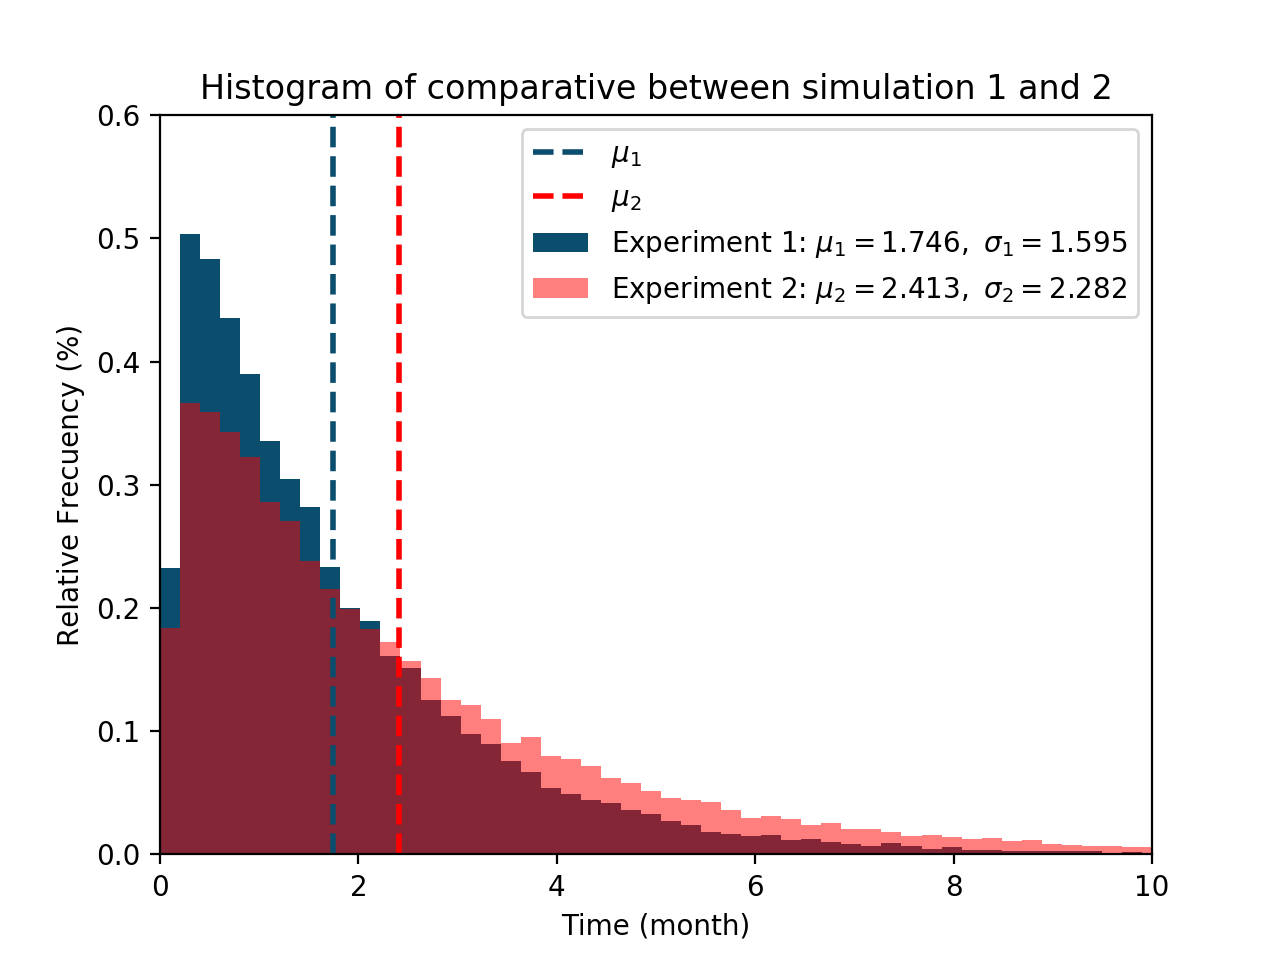
\includegraphics[scale=1.1]{graphics/Comparative_graphic_1.png}
      \caption{Comparación simulaciones 1 y 2}
      \centering
    \end{figure}

    \par Podemos apreciar en la \textit{Figura 1} que existe una ganancia aproximada de un mes de la simulación con un
    operario más sobre la representación del sistema incial. Dicho resultado es el esperado, dado que la velocidad de
    reparación de una máquina es mayor pues aumenta la cantidad de trabajadores encargados de dicha tarea.

  \pagebreak
  \subsection{\underline{Comparación 2:} Simulaciones 1 y 3}

    \par Al igual que en la comparación anterior, el objetivo del siguiente gráfico entre el sistema original y la
    simulación con una máquina de repuesto más, es dejar en evidencia cual es la mejoría, en caso que existiese, en el
    agregado de un operario en el sistema de la lavandería.

    \begin{figure}[H]
      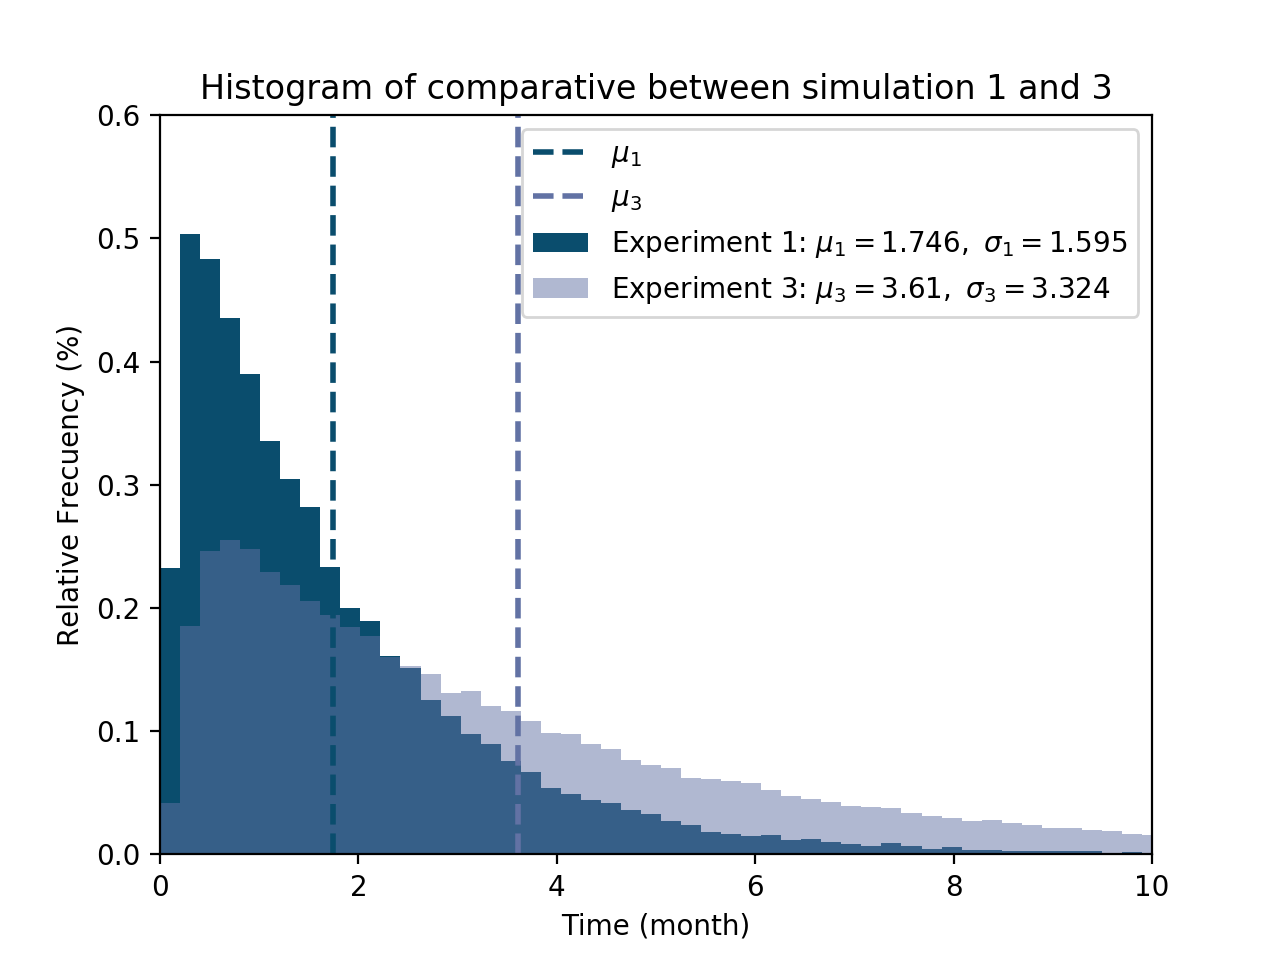
\includegraphics[scale=1.1]{graphics/Comparative_graphic_2.png}
      \caption{Comparación simulaciones 1 y 3}
      \centering
    \end{figure}

    \vspace{5mm}
    \par Similarmente a los ocurrido en la comparación anterior, se puede apreciar una mejoría de la simulación con una
    máquina de repuesto más, sobre la representación del sistema inicial. Dicha mejoría es aún mayor que en la anterior
    comparación, dado que este mismo suceso ocurre con los valores esperados de las simulaciones, es decir, la
    esperanza del segundo sistema es mayor que la del primero. Numéricamente esta diferencia ronda los dos meses.
    Nuevamente, este resultado es el esperado, dado que en el momento que ocurriese un fallo en alguna de las máquinas,
    se contará con un repuesto más que en sistema inicial.

  \pagebreak
  \subsection{\underline{Comparación 3:} Simulaciones 2 y 3}

    \par En el esquema correlativo, podemos apreciar las diferencias existentes entre las dos posibles soluciones a la
    mejora del sistema original. Es decir, se comparan los histogramas resultantes de las
    simulaciones con dos máquinas de repuesto y un operario contra tres máquinas y un operario.

    \begin{figure}[H]
      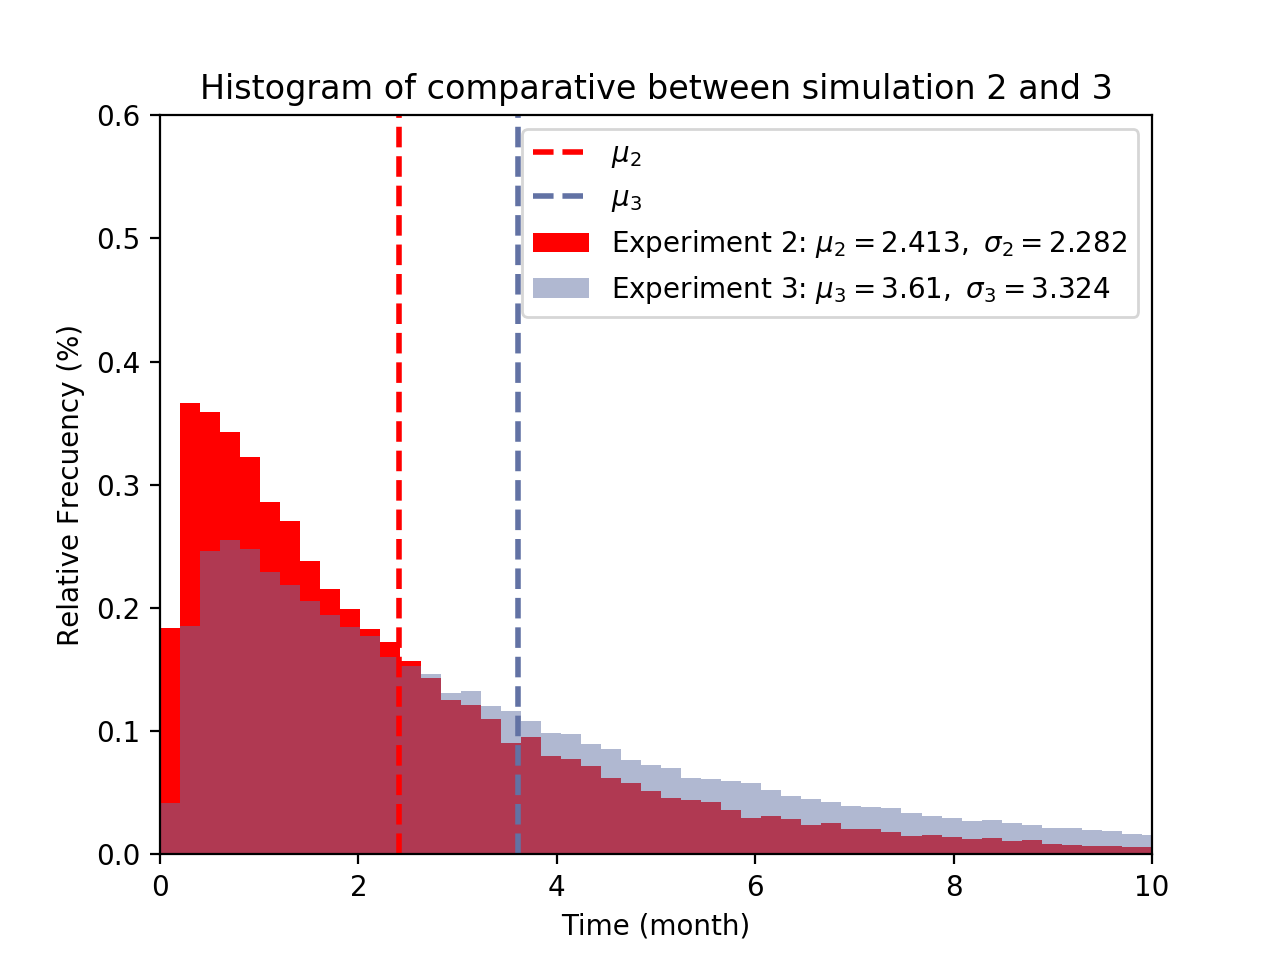
\includegraphics[scale=1.1]{graphics/Comparative_graphic_3.png}
      \caption{Comparación simulaciones 2 y 3}
      \centering
    \end{figure}

    \par Dado que, como se observo en las \textit{Figura 1} y \textit{Figura 2}, existe una diferencia cercana al mes
    entre los valores de las simulaciones con uno y dos operarios, y de dos meses entre las representaciones con dos y
    tres máquinas de repuesto, este histograma muestra una desigualdad cercana al mes entre los tiempos de vida
    esperados de dichas simulaciones.

  \pagebreak
  \subsection{\underline{Extrapolación en 3D}}

    \par Por último, el siguiente figura, realizado en tres dimesiones, tiene como objetivo acentuar las conclusiones
    ya realizadas en las secciones y gráficos anteriores, esto es, dejar en evidencia que en ambos casos, es decir,
    agregando ya sea operarios o máquinas el sistema mejorará, pero dicha mejora será aún mayor en la simulación que
    adicione máquinas.

    \begin{figure}[H]
      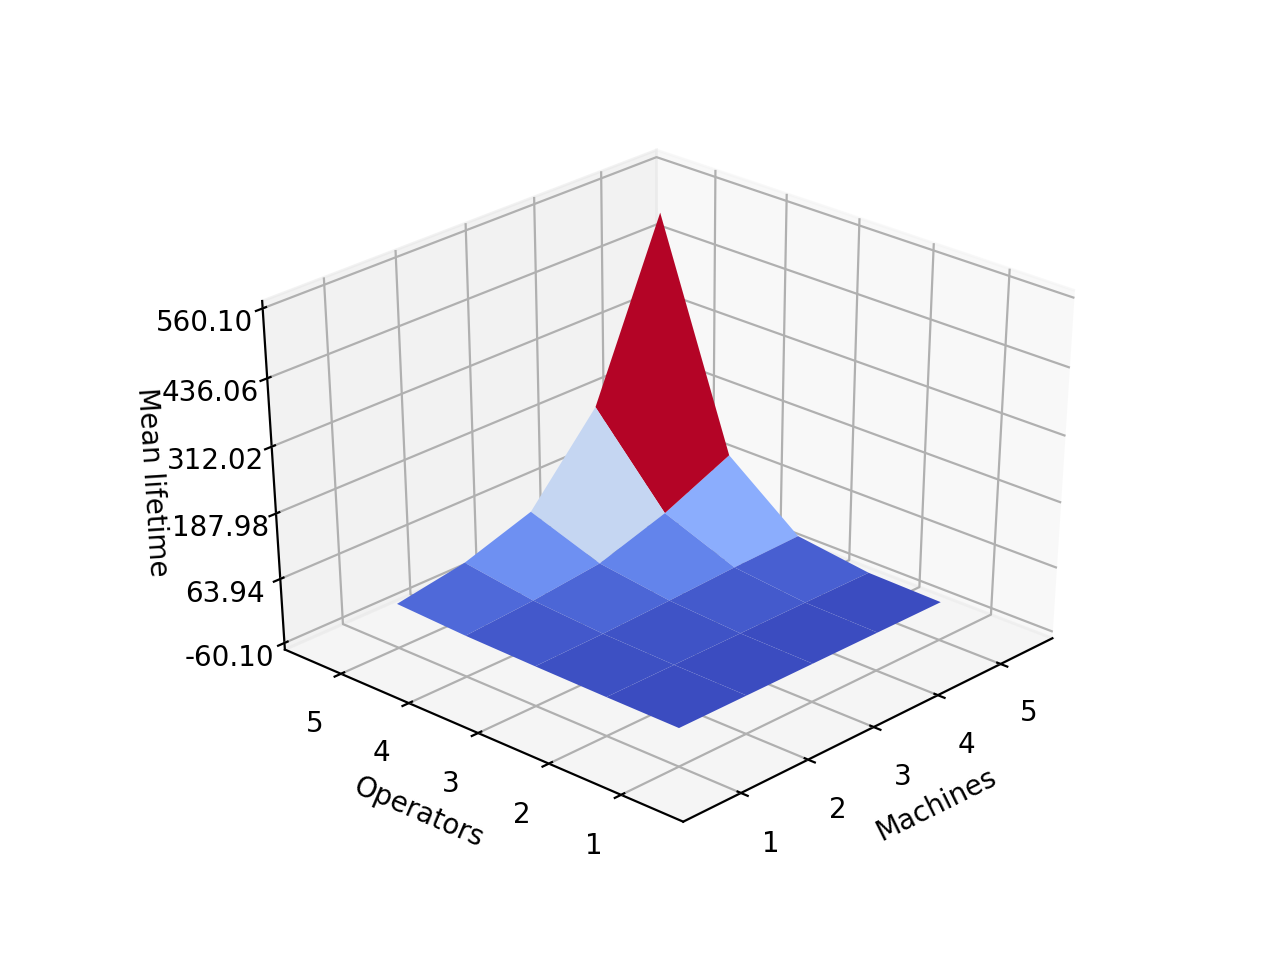
\includegraphics[scale=1.2]{graphics/Figure_4.png}
      \caption{Simulación en 3D}
      \centering
    \end{figure}

  \pagebreak
  \subsection{Tablas comparativas entre simulaciones}

    \par Los consecuentes resultados pertenecen a los tres sistemas simulados y recientemente desarrollados. Dichos
    valores se corresponden con un intervalo de confianza del 99 \%.

    \begin{itemize}
      \item \textbf{Figura 1: 5 máquinas funcionando, 2 máquinas de repuesto y 1 operario}
        \begin{center}
          \begin{tabular}{| l | l | l | l |}
          \hline
            Confianza & $\mu$ & $\sigma^2$ & $\sigma$ \\\hline\hline
            99 \% & 1.746 & 2.545 & 1.595 \\\hline
          \end{tabular}
        \end{center}
      \vspace{5mm}
      \item \textbf{Figura 2: 5 máquinas funcionando, 2 máquinas de repuesto y 2 operarios}
        \begin{center}
          \begin{tabular}{| l | l | l | l |}
          \hline
            Confianza & $\mu$ & $\sigma^2$ & $\sigma$ \\\hline\hline
            99 \% & 2.413 & 5.208 & 2.282 \\\hline
          \end{tabular}
        \end{center}
      \vspace{5mm}
      \item \textbf{Figura 3: 5 máquinas funcionando, 3 máquinas de repuesto y 1 operario}
        \begin{center}
          \begin{tabular}{| l | l | l | l |}
          \hline
            Confianza & $\mu$ & $\sigma^2$ & $\sigma$ \\\hline\hline
            99 \% & 3.610 & 11.049 & 3.324 \\\hline
          \end{tabular}
        \end{center}
    \end{itemize}


\pagebreak

\section{Conclusión}

  \par Partiendo del problema presentado en la introducción de este informe, se analizaron dos posibles mejoras sobre
  el sistema inicial. Las mismas consistieron, por un lado, en el agregado de una máquina de repuesto, mientras que por
  el otro, el yuxtapuesto de un operario.

  \par Luego de simular las mejoras recientemente mencionadas, podemos concluír que añadir un operario mejora
  escuetamente el funcionamiento esperado del sistema. En lo que respecta a números, la esperanza de vida del mismo
  aumenta en un tiempo cercano al mes. Mientras que lo mismo ocurre con las frecuencias relativas del sistema simulado,
  por lo que la curva en su totalidad muestra un perfeccionamiento respecto al sistema inicial.

  \par Por otro lado, se observa que resulta más conveniente añadir una lavadora de repuesto sobre agregar un operario,
  puesto que la esperanza de un sistema con dos operarios es menor que la de uno que cuenta con tres máquinas de
  respuesto. Refiriendonos a tiempo, las esperanzas difieren aproximadamente en un tiempo de dos meses. Además, podemos
  observar que las frecuencias relativas se concentran con mayor reiteración cercanas a la media, en el sistema con dos
  operarios, mientras que se distribuyen uniformemente a lo largo de la recta en el sistema con tres máquinas de
  reserva. Luego, en las simulaciones realizadas con un operario y dos o tres máquinas de repuesto, se apreciaron
  resultados similares a los ya contemplados con anterioridad.

  \par Finalmente, como apreciación personal, consideramos que este tipo de simulaciones son muy beneficiosas, ya que
  posibilitan la modelización de posibles modificaciones a sistemas como el de la lavandería. Esto permite observar
  como reacciona el sistema frente a dichas modificaciones para que luego, a partir de estos resultados se tomen las
  elecciones que mejor se adecuén a los objetivos propuestos.


\pagebreak

\end{document}
